\chapter{Theoretical Basis for CFAST}

Adequately detailed documentation of the theoretical basis of the model allows the model user to
understand the underlying theory behind the model implementation and thus be able to assess the
appropriateness of the model to specific problems. This chapter presents a derivation of the
predictive equations for zone fire models and explains in detail the ones used in CFAST.

The modeling equations used in CFAST take the mathematical form of an initial value problem
for a system of ordinary differential equations. These equations are derived using the
conservation of mass, the conservation of energy (equivalently the first law of thermodynamics),
the ideal gas law. These equations predict as functions of time quantities such as pressure, layer
height and temperatures given the accumulation of mass and enthalpy in the two layers. The
assumption of a zone model is that properties such as temperature can be approximated
throughout a control volume by an average value.

Many formulations based upon these assumptions can be derived. One formulation can be
converted into another using the definitions of density, internal energy and the ideal gas law.
Though equivalent analytically, these formulations differ in their numerical properties. Each
formulation can be expressed in terms of mass and enthalpy flow. These rates represent the
exchange of mass and enthalpy between zones due to physical phenomena such as plumes,
natural and forced ventilation, convective and radiative heat transfer, and so on. For example, a
vent exchanges mass and enthalpy between zones in connected rooms, a fire plume typically
adds heat to the upper layer and transfers entrained mass and enthalpy from the lower to the
upper layer, and convection transfers enthalpy from the gas layers to the surrounding walls.

As discussed in references \cite{Forney:1994} and \cite{Rehm:1992}, the zone fire modeling ordinary differential equations (ODEs) are stiff. The term stiff means that large variations in time scales are present in the ODE solution. In our problem, pressures adjust to changing conditions more quickly than other to solve zone fire modeling ODEs because of this stiffness. Runge-Kutta methods or predictor-corrector methods such as Adams-Bashforth require prohibitively small time steps in order to
track the short-time scale phenomena (pressure in our case). Methods that calculate the Jacobian
(or at least approximate it) have a much larger stability region for stiff problems and are thus
more successful at their solution.

\section{Derivation of Equations for a Two-Layer Model}

A compartment is divided into two control volumes, a relatively hot upper layer and a relatively cool lower layer, as illustrated in figure \ref{fig:Control_Volumes}.  The gas in each layer has attributes of mass, internal energy, density, temperature, and volume denoted respectively by $m_i$, $E_i$, $\rho_i$, $T_i$, and $V_i$ where $i$=$L$ for the lower layer and $i$=$U$ for the upper layer.  The compartment as a whole has the attribute of pressure $P$.  These 11 variables are related by means of the following seven constraints (counting density, internal energy and the ideal gas law twice, once for each layer).

\be \rho _i  = \frac{{m_i }}{{V_i }} {\hspace{1.0in} \textnormal{Density}} \label{eq:density} \ee

\be  E_i = c_v m_i T_i {\hspace{1.0in} \textnormal{Internal Energy}} \label{eq:internal_energy} \ee

\be P = R\rho _i T_i {\hspace{1.0in} \textnormal{Ideal Gas Law}} \ee

\be V = V_L + V_U {\hspace{1.0in} \textnormal{Total Volume}} \label{eq:volume} \ee

\begin{figure}[h]
\begin{center}
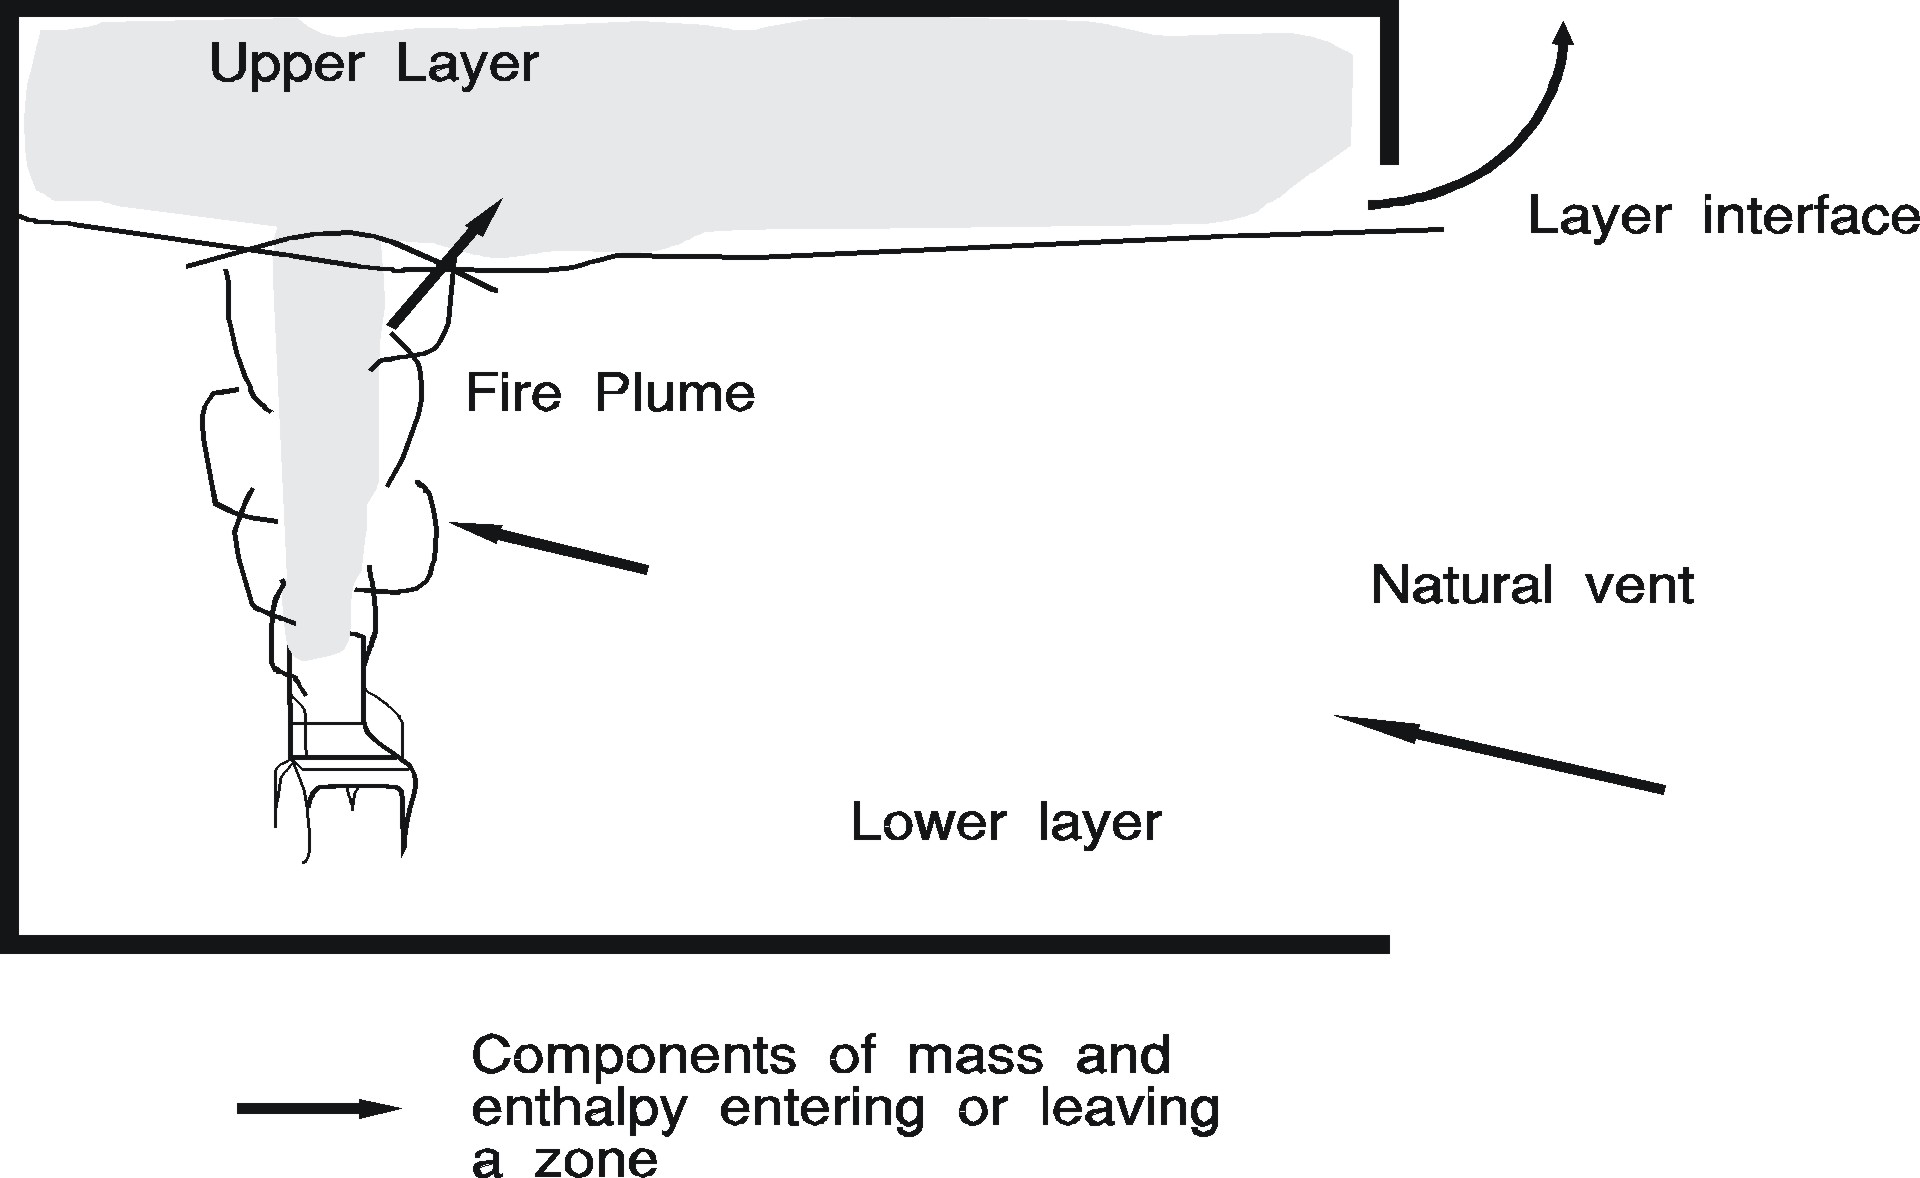
\includegraphics[width=4.0in]{FIGURES/Theory/Control_Volumes}\\
\end{center}
\caption{Schematic of control volumes in a two-layer zone model.}
 \label{fig:Control_Volumes}
\end{figure}

The specific heat at constant volume and at constant pressure $c_v$ and cp, the universal gas constant, R, and the ratio of specific heats, $\gamma$, are related by $\gamma = c_p / c_v$ and $R = c_p- c_v$.  For ambient air, $c_p \approx 1$ kJ/kg K and $\gamma = 1.4$.  Four additional equations obtained from conservation of mass and energy for each layer are required to complete the equation set.  The differential equations for mass in each layer are 

\be \frac{{dm_L }}{{dt}} = \dot m_L \ee

\be \frac{{dm_U }}{{dt}} = \dot m_U \ee

The first law of thermodynamics states that the rate of increase of internal energy plus the rate at
which the layer does work by expansion is equal to the rate at which enthalpy is added to the gas.
In differential form this is

\be \begin{array}{ccccc}
   {{\textnormal{internal energy}}} & {} & {{\textnormal{work}}} & {} & {{\textnormal{enthalpy}}}  \\
   {\overbrace {}^{}} & {} & {\overbrace {}^{}} & {} & {\overbrace {}^{}}  \\
   {\displaystyle {\dbydt{E_i}}} &  +  & {P \displaystyle {\dbydt{V_i}}} &  =  & {\dot h_i }  \\
\end{array} \label{eq:first_law} \ee

where $c_p$ is taken as constant in the enthalpy term,

\be \dot h = c_p \dot m_U T_U + \dot E_U + c_p \dot m_LT_L + \dot E_L \ee

A differential equation for pressure can be derived by adding the upper and lower layer versions
of eq (\ref{eq:first_law}), noting that $\dbydt{V_U} = -\dbydt{V_L}$, and that

\be \dbydt{E_i} = \dbydt{ \brackets{c_v \dot m_i T_i}} = \frac{{c_v}}{{R}} \dbydt{ \brackets{PV_i}} \label{eq:differential_internal_energy}  \ee

to obtain

\be \dbydt{P} = \frac{{\gamma -1}}{{V}} \brackets{\dot h_L + \dot h_U}  \ee

Differential equations for the layer volumes can be obtained by substituting equation \ref{eq:differential_internal_energy} into \ref{eq:first_law} to obtain

\be \dbydt{V_i} = \frac{1}{P \gamma} \brackets{\brackets{\gamma -1} \dot h_i - V_i \dbydt{P}} \label{eq:layer_volume} \ee

Equation \ref{eq:internal_energy} can be rewritten using eq \ref{eq:layer_volume} to eliminate $dV/dt$ to yield

\be \dbydt{E_i} = \frac{1}{\gamma} \brackets{\dot h_i + V \dbydt{P}} \ee

A differential equation for density can be derived by applying the quotient rule to $\frac{d \rho_i}{dt} = \frac{d}{dt} \brackets{\frac{m_i}{V_i}}$ and using eq \ref{eq:layer_volume} to eliminate $\frac{dV_i}{dt}$ to obtain

\be \dbydt{\rho_i} = \frac{-1}{c_p T_i V_i} \brackets{\brackets{\dot h_i - c_p \dot m_i T_i} - \frac{V_i}{\gamma - 1}\dbydt{P}} \label{eq:layer_density}\ee

Temperature differential equations can be obtained from the equation of state by applying the quotient rule to $\dbydt{T_i} = \dbydt{} \brackets{\frac{P}{R \rho_i}}$ and using eq \ref{eq:layer_density} to eliminate $\dbydt{\rho_i}$ to obtain

\be \dbydt{T_i} = \frac{1}{c_p rho_i V_i} \brackets{\brackets{\dot h_i - c_p \dot m_i T_i}+ V_i \dbydt{P}} \ee

These equations for each of the 11 variables are summarized in table \ref{tab:zone_model_equations}. The time evolution of
these solution variables can be computed by solving the corresponding differential equations
together with appropriate initial conditions. The remaining seven variables can be determined
from the four solution variables using eqs (\ref{eq:density}) to (\ref{eq:volume}).

\begin{table}
\begin{center}
\caption{Conservative zone model equations}
\label{tab:zone_model_equations}
\vspace{0.1in}
\begin{tabular}{|c|c|}
\hline
Equation Type & Differential Equation \\ \hline
i'th layer mass & $\displaystyle {\dbydt{m_i} = \dot m_i}$ \\ \hline
pressure & $\displaystyle {\dbydt{P} = \frac{{\gamma -1}}{{V}} \brackets{\dot h_L + \dot h_U}}$ \\ \hline
i'th layer energy & $\displaystyle {\dbydt{E_i} = \frac{1}{\gamma} \brackets{\dot h_i + V \dbydt{P}}}$ \\ \hline
i'th layer volume & $\displaystyle {\dbydt{V_i} = \frac{1}{P \gamma} \brackets{\brackets{\gamma -1} \dot h_i - V_i \dbydt{P}} }$ \\ \hline
i'th layer density & $\displaystyle {\dbydt{\rho_i} = \frac{-1}{c_p T_i V_i} \brackets{\brackets{\dot h_i - c_p \dot m_i T_i} - \frac{V_i}{\gamma - 1}\dbydt{P}}}$ \\ \hline
i'th layer temperature & $\displaystyle {\dbydt{T_i} = \frac{1}{c_p rho_i V_i} \brackets{\brackets{\dot h_i - c_p \dot m_i T_i}+ V_i \dbydt{P}}}$ \\ \hline
\end{tabular}  
\end{center}
\end{table}

There are, however, many possible differential equation formulations. Indeed, there are 330
different ways to select four variables from eleven. Many of these systems are incomplete due to
the relationships that exist between the variables given in eqs (\ref{eq:density}) to (\ref{eq:volume}). For example the
variables, $\rho_U$, $V_U$, $m_U$, and $P$ form a dependent set since $\rho_U = m_U / V_U$.

The number of differential equation formulations can be considerably reduced by not mixing
variable types between layers; that is, if upper layer mass is chosen as a solution variable, then
lower layer mass must also be chosen. For example, for two of the solution variables choose $m_L$
and $m_U$, or $\rho_L$ and $\rho_U$, or $T_L$ and $T_U$. For the other two solution variables pick $E_L$ and $E_U$ or $P$ and $V_L$ or $P$ and $V_U$. This reduces the number of distinct formulations to nine. Since the numerical properties of the upper layer volume equation are the same as a lower layer one, the number of
distinct formulations can be reduced to six.

\section{Equation Set Used in CFAST}

The current version of CFAST is set up to use the equation set for layer temperature, layer
volume, and pressure as shown below.

\be \dbydt{P} = \frac{{\gamma -1}}{{V}} \brackets{\dot h_L + \dot h_U}  \ee

\be \dbydt{V_U} = \frac{1}{P \gamma} \brackets{\brackets{\gamma -1} \dot h_i - V_U \dbydt{P}} \ee

\be \dbydt{T_U} = \frac{1}{c_p rho_i V_U} \brackets{\brackets{\dot h_U - c_p \dot m_U T_U}+ V_U \dbydt{P}} \ee

\be \dbydt{T_L} = \frac{1}{c_p rho_i V_L} \brackets{\brackets{\dot h_L - c_p \dot m_L T_L}+ V_L \dbydt{P}} \ee

In these equations, the pressure is actually modeled with the pressure difference relative to an
ambient reference pressure to minimize numerical instability.

\section{Limitations of the Zone Model Assumptions}

The basic assumption of all zone fire models is that each compartment can be divided into a
small number of control volumes, each of which is uniform in temperature and composition. In
CFAST all compartments have two zones except for the fire room which has an additional zone
for the plume. Since a real upper/lower interface is not as sharp as this, one has a spatial error of
about 10~\% in determining the height of the layer \cite{Steckler:1982, Quintiere:1984}.

The zone model concept best applies for an enclosure in which the width and length are not too
different. If the horizontal dimensions of the room differ too much (i.e., the room looks like a
corridor), the flow pattern in the room may become asymmetrical. If the enclosure is too
shallow, the temperature may have significant radial differences. The width of the plume may at
some height become equal to the width of the room and the model assumptions may fail in a tall
and narrow enclosure. Therefore, the user should recognize approximate limits on the ratio of the
length ($L$), width ($W$), and height ($H$) of the compartment.

If the aspect ratio (length/width) is over about 10, the corridor flow algorithm should be used.
This provides the appropriate filling time. Similarly, for tall shafts (elevators and stairways), a
single zone approximation is more appropriate. It was found experimentally \cite{Klote:1990} that the mixing
between a plume and lower layer due to the interaction with the walls of the shaft, caused
complete mixing. The is the flip side of the corridor problem and occurs at a ratio of the height
to characteristic floor length of about 10. The following quantitative limits are recommended:

\begin{table}[h]
\begin{center}
\caption{Recommended compartment dimension limits}
\label{tab:compartment_limits}
\vspace{0.1in}
\begin{tabular}{|c|c|c|c|}
\hline
Group & Acceptable & Special consideration & Corridor flow \\ 
 & & required & algorithm \\ \hline
$(L/W)_{max}$ & $L/W < 3$ & $3 < L/W < 5$ & $L/W > 5$ \\ \hline
$(L/H)_{max}$ &  $L/H < 3$ & $3 < L/H < 6$ & $L/H > 6$ \\ \hline
 $(W/H)_{max}$ & $W/H > 0.4$ & $0.2 < L/W < 0.4$ & $L/W < 0.2$ \\ \hline
\end{tabular}  
\end{center}
\end{table}

\section{Source Terms for the Model}

This section discusses each of the sub-models in CFAST. In general, the sections are similar to
the way the model itself is structured. The sub-sections which follow discuss the way the actual
phenomena are implemented numerically. For each of the phenomena discussed below, the
physical basis for the model is discussed first, followed by a brief presentation of the
implementation within CFAST. For all of the phenomena, there are basically two parts to the
implementation: the physical interface routine (which is the interface between the CFAST
model and the algorithm) and the actual physical routine(s) which implement the physics. This
implementation allows the physics to remain independent of the structure of CFAST and allows
easier insertion of new phenomena.

\subsection{The Fire}

A fire in CFAST is implemented as a source of fuel mass which is released at a prescribed rate
(the pyrolysis rate). Energy is released by the fuel and combustion products are created as it
burns.

The model can simulate multiple fires in one or more compartments of the building. These fires
are treated as totally separate entities, with no interaction of the plumes. These fires are generally
referred to as ``objects'' and can be ignited at a prescribed time, temperature or heat flux.

CFAST does not include a pyrolysis model to predict fire growth. Rather, pyrolysis rates for
each fire are prescribed by the user. While this approach does not directly account for increased
pyrolysis due to radiative feedback from the flame or compartment, in theory these effects could
be prescribed by the user. In an actual fire, this is an important consideration, and the
specification used should consider the experimental conditions as closely as possible.

\subsubsection{Constrained Fire}

A fire releases energy based on the pyrolysis of fuel, but may be constrained by the oxygen
available for combustion depending on the compartment conditions. Complete burning will take
place only where there is sufficient oxygen. When insufficient oxygen is entrained into the fire
plume, unburned fuel will be transported from zone to zone until there is sufficient oxygen and a
high enough temperature to support combustion. In general, CFAST uses a simple definition of
a combustion reaction that includes major products of combustion for hydrocarbon fuels:

\be  \mathrm{C_xH_yO_zN_aCl_b} +  \nu_\OTWO \, \mathrm{O_2}  \rightarrow  \nu_\COTWO \, \mathrm{CO_2} + \nu_\HTWOO \, \mathrm{H_2O} + \nu_\CO \, \mathrm{CO} +
     \nu_\So \, \mathrm{Soot}  + \nu_\NTWO \, \mathrm{N_2} + \nu_\HCl \mathrm{HCl} + \nu_\HCN \mathrm{HCN} \label{stoich} \ee     
where the stoichiometric coefficients $\nu\OTWO$, $\nu_\COTWO$, etc. represent appropriate molar ratios for a stoichiometric balance of the equation.  For example, for soot, it is related to the
{\em soot yield}, $y_\So$, via the relation:
\be
   \nu_\So = \frac{W_\F}{W_\So} \; y_\So \label{soot_yield}
\ee

For complete combustion of the simplest hydrocarbon fuel, methane reacts with 
oxygen to form carbon dioxide and water. The only input required is the pyrolysis rate and the 
heat of combustion. For fuels that contain oxygen, nitrogen, or chlorine, the reaction becomes 
more complex. In this case, production yields for the species are prescribed by the user. 
Stoichiometry is used to insure conservation of mass and elements in the reaction. The species 
which are calculated are oxygen, carbon dioxide, carbon monoxide, water, and soot. Gaseous nitrogen is included, but only acts as a diluent. Production of hydrogen cyanide and hydrogen chloride are tracked solely based on user prescribed yields. The heat release rate for a constrained fire may be reduced below its prescribed value based upon the oxygen available for combustion.  When there is not enough oxygen to support complete combustion, some of the fuel will be transported to the gas layers and through vents as unburned hydrocarbons.

As fuel and oxygen are consumed, heat is released and various products of combustion are formed. The heat is released as radiation and convected enthalpy:

\begin{eqnarray} Q_{f,R} &=& \chi_R Q_f \\
Q_{f,R} &=& \brackets{1-\chi_R} Q_f
\end{eqnarray}
where, $\chi_R$ is the fraction  of the fire�s heat release rate given off as radiation.  The convective 
enthalpy, $Q_{f,C}$ then becomes the driving term in the plume flow.  For a constrained fire there is 
radiation to both the upper and lower layers, whereas the convective part contributes only to the 
upper layer.

\subsubsection{Limiting Combustion by Available Oxygen}

For any individual fire, the heat release rate is limited by available oxygen in the layer where the fire is located. This limit is applied in three 
places, which are shown schematically in figure 3. The first is burning in the portion of the 
plume which (at least initially) is typically in the lower layer of the room of fire origin (region \# 1).  The second is the portion of the plume in the upper layer, also in the room of origin (region \# 2).  The third is in the 
vent flow which entrains air from a lower layer into an upper layer in an adjacent compartment 
(region \# 3). The unburned hydrocarbons are tracked in this model.  Further combustion of CO to 
$\mathrm{CO_2}$ is not included in the model.

\begin{figure}[h]
\begin{center}
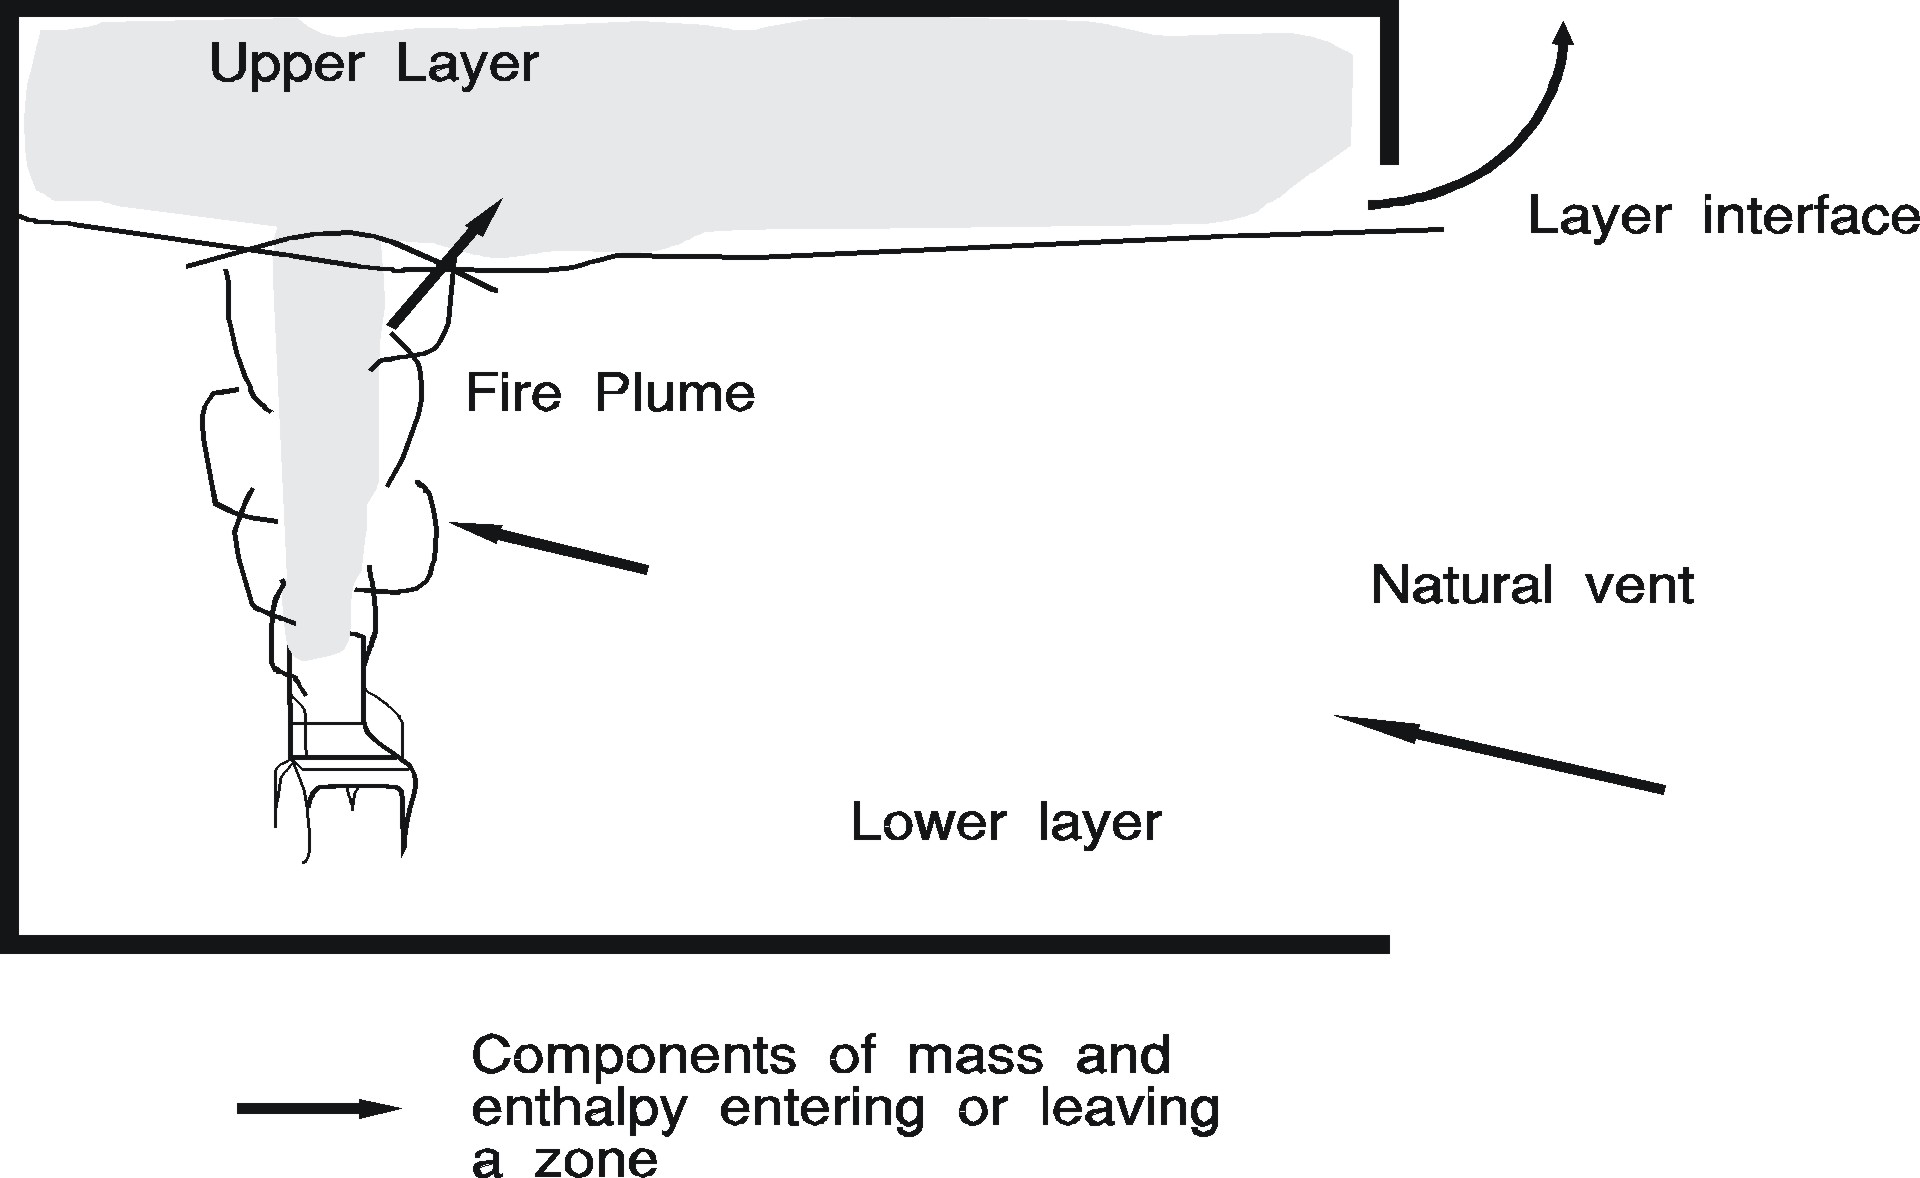
\includegraphics[width=4.0in]{FIGURES/Theory/Control_Volumes}\\
\end{center}
\caption{Entrainment and burning in a two-layer, multi-compartment model.}
 \label{fig:Burning_Regions}
\end{figure}

Initially, $\dot{m_f}$ is just the pyrolysis rate of the source fire in kg/s (region \# 1). For subsequent regions, the burning rate $\dot{m_f}$ is the unburned fuel from a previous region, $\dot{m_{tuhc}} = \dot{m_f} - \dot{m_b}$ where the subscript $tuhc$ is total unburned hydrocarbons, $f$ is the fire source, and $b$ is the amount burned.

The first step is to limit the actual burning which takes place in the combustion zone.  In each 
combustion zone, there is a quantity of fuel available.  At the source this results from the 
pyrolysis of the material, $\dot{m}_f$ .  In other situations such as a plume or door jet, it is the net 
unburned fuel available, $\dot{m}_{tuhc}$.  In each case, the fuel which is available but not burned is then 
deposited into the ``$\dot{m}_{tuhc}$ '' category.  This provides a consistent notation.  In the discussion below, 
$\dot{m}_f$  is the amount of fuel burned.  This value is initially specified as to the available fuel, and then 
reduced if there is insufficient oxygen to support complete combustion.  Subsequently, the 
available fuel, $\dot{m}_{tuhc}$, is reduced by the final value of $\dot{m}_f$ burned or $\dot{m}_b$.  Thus we have a consistent description in each burning region, with an algorithm that is invoked independent of the region being analyzed.

\be Q = \dot{m}_f H_c \ee
with the mass of oxygen required to achieve this energy release rate of
\be \dot{m}_O = \frac{Q}{E} = \dot{m}_f \frac{H_c}{E} \ee
where $E$ is the heat release per mass unit of oxygen consumed, taken to be 1.31 x $10^7$ J/kg\footnote{The units for oxygen consumption calorimetry are J/kg. The value 1.31 x $10^7$ J/kg is representative of typical fuels such as furniture (see reference \cite{Morehart:1991}) and implies these units. The variation or uncertainty (2$\sigma$) associated with this value is on the order of $\pm$ 5 \%} (based 
on oxygen consumption calorimetry for typical fuels \cite{Morehart:1991, Thornton:1917, Huggett:1980}). If the fuel contains oxygen (available for combustion), the oxygen needed to achieve full combustion is less:

\be \dot{m}_{O,needed} = \dot{m}_O - \dot{m}_{O, in the fuel} \ee

If sufficient oxygen is available, then it is fully burned.  However, if the oxygen concentration is 
low enough, it will constrain the burning and impose a limit on the amount of fuel actually 
burned, as opposed to the amount pyrolyzed.  The actual limitation is discussed below and is:

\be \dot{m}_{O.actual} = min \brackets{\dot{m}_{O,available} , \dot{m}_{O,needed}} \ee

\be \dot{m}_{f,actual} = \dot{m}_{O,actual} \frac{E}{H_c}  \ee
The relationship between oxygen and fuel concentration defines a range in which burning will 
take place.  In the CFAST model, a limit is incorporated by limiting the burning rate as the 
oxygen level decreases until a ``lower oxygen limit'' (LOL) is reached. The lower oxygen limit is 
incorporated through a smooth decrease in the burning rate near the limit:

\be \dot{m}_{O,available} = \dot{m}_eY_{O_2}C_{LOL} \ee
where $\dot{m}_e$ is the mass entrainment flow rate, $Y_{O_2}$ is the mass fraction of oxygen, and the lower oxygen limit coefficient, $C_{LOL}$  
, is the fraction of the available fuel which can be burned with the 
available oxygen and varies from 0 at the limit to 1 above the limit.  The functional form that 
utilizes the hyperbolic tangent was determined empirically to provide a smooth cutoff of the 
burning over a narrow range above the limit.

\be C_{LOL} = \frac{\tanh\brackets{{800 \brackets{Y_{O_2} - Y_{LOL}} - 400}} + 1}{2} \ee
A temperature criterion is also imposed so that no burning will take place when the temperature 
is below a user prescribed temperature.

In summary, it is possible to follow the formation of the major products of combustion (carbon 
dioxide, carbon monoxide, soot, water, hydrogen cyanide, and hydrogen chloride) using 
appropriate measured product yields (e.g., \cite{Morehart:1991}) to define product yields for eq (33). Actual 
combustion chemistry is not considered in CFAST due to the complexities associated with 
detailed kinetics and transport. 

\subsubsection{Flame Height}

CFAST includes a calculation of average flame height based on the work of Heskestad \cite{Heskestad:2002}. 
Valid for a wide range of hydrocarbon and gaseous fuels, the correlation is given by

\be H = -1.02 D + 0.235 \brackets{\frac{Q_f}{1000}} \ee
where $H$ is the average flame height, $D$ the diameter of the fire and $Q_f$ is the fire size. The mean 
flame height is defined as the distance from the fuel source to the top of the visible flame where 
the intermittency is 0.5.  A flame intermittency of 0.5 means that the visible flame is above the 
mean 50 \% of the time and below the mean 50 \% of the time.  This average flame height is 
 included in the printed output from CFAST. Note that $Q_f$ in Eq. (8) in Ref. \cite{Heskestad:2002} is in kW.
 
 \subsubsection{Limitation of the Algorithm for Fires and Mass Balance }
 
CFAST depends on pyrolysis data for the source term for a fire. The usual way to obtain this 
data is a large-scale calorimeter, e.g., reference [\cite{Bryant:2003}. Generally, a product (e.g., chair, table, 
bookcase) is placed under a large collection hood and ignited by a burner ($\approx 50$ kW simulating a wastebasket) placed adjacent to the item.  The combustion process then proceeds under assumed 
�free-burning� conditions, and the heat release rate is measured.  Potential sources of uncertainty 
include measurement errors related to the instrumentation and the degree to which �free-burn- 
ing� conditions are not achieved (e.g., radiation from the gases under the hood or from the hood 
itself, and restrictions in the air entrained by the object causing locally reduced oxygen 
concentrations affecting the combustion chemistry).  There are limited experimental data for 
upholstered furniture which suggest that prior to the onset of flashover in a compartment, the 
influence of the compartment on the burning behavior of the item is small.  The differences 
obtained from the use of different types or locations of ignition sources have not been explored. 
These factors are discussed in reference~\cite{Babrauskas:1982}. 

Where small-scale calorimeter data are used, procedures are available to extrapolate to the 
behavior of a full-size item.  These procedures are based on empirical correlations of data which 
exhibit significant scatter, thus limiting their accuracy.  For example, for upholstered furniture, 
the peak heat release rates estimated by the �triangular approximation� method averaged 91 \% 
(range 46 \% to 103 \%) of values measured for a group of 26 chairs with noncombustible frames, 
but only 63 \% (range 46 \% to 83 \%) of values measured for a group of 11 chairs with 
combustible frames \cite{Babrauskas:1985}.  Also, the triangle neglects the �tails� of the curve; these are the initial time from ignition to significant burning of the item, and the region of burning of the combusti- 
ble frame, after the fabric and filler are consumed. 

The provided data and procedures only relate directly to burning of items initiated by relatively 
large flaming sources.  Little data are currently available for release rates under smoldering 
combustion, or for the high external flux and low oxygen conditions characteristic of post- 
flashover burning.  While the model allows multiple items burning simultaneously, it does not 
account for the synergy of such multiple fires.  Thus, for other ignition scenarios, multiple items 
burning simultaneously (which exchange energy by radiation and convection), combustible 
interior finish, and post-flashover conditions, the model can give estimates which are often non- 
conservative (the actual release rates would be greater than estimated).  At present, the only sure 
way to account for all of these complex phenomena is to conduct a full-scale compartment burn 
and use the pyrolysis rates directly. 

Burning can be constrained by the available oxygen.  However, this �constrained fire� is not 
subject to the influences of radiation to enhance its burning rate, but is influenced by the oxygen 
available in the compartment.  If a large mass loss rate is entered, the model will follow this 
input until there is insufficient oxygen available for that quantity of fuel to burn in the 
compartment.  The unburned fuel (sometimes called excess pyrolysate) is tracked as it flows out 
in the door jet, where it can entrain more oxygen.  If this mixture is within the user-constrained 
flammable range, it burns in the door plume.  If not, it will be tracked throughout the building 
until it eventually collects as unburned fuel or burns in a vent.  The enthalpy released in the fire 
compartment and in each vent, as well as the total enthalpy released, is detailed in the output of 
the model.  Since mass and enthalpy are conserved, the total will be correct.  However, since 
combustion did not take place adjacent to the burning object, the actual mass burned could be 
lower than that specified by the user.  The difference will be the unburned fuel. 

An oxygen combustion chemistry scheme is employed only in constrained fires.  Here user- 
constrained hydrocarbon ratios and species yields are used by the model to predict concentra- 
tions.  A balance among hydrogen, carbon, and oxygen molecules is maintained.  Under some 
conditions, low oxygen can change the combustion chemistry, with a resulting increase in the 
yields of products of incomplete combustion such as carbon monoxide. However, not enough is 
known about these chemical processes to build this relationship into the model at the present 
time.  Some data exist in reports of full-scale experiments (e.g., reference \cite{Lee:1982}) which can assist in making such determinations.

\subsection{Plumes} 

A plume is formed above any burning object.  It acts as a pump transferring mass and enthalpy 
from the lower layer into the upper layer.  A correlation is used to predict the amount of mass 
and enthalpy that is transferred.  A more complete plume model would predict plume 
entrainment by creating a separate zone and solving the appropriate equations.

Two sources exist for moving enthalpy and mass between the layers within and between 
compartments.  Within the compartment, the fire plume provides one source.  The other source 
of mixing between the layers occurs at vents such as doors or windows.  Here, there is mixing at 
the boundary of the opposing flows moving into and out of the compartment.  The degree of 
mixing is based on an empirically-derived mixing relation.  Both the outflow and inflow entrain 
air from the surrounding layers.  The flow at vents is also modeled as a plume (called the door 
plume or jet), and uses the same equations as the fire plume, with two differences.  First, an 
offset is calculated to account for entrainment within the doorway and second, the equations are 
modified to account for the rectangular geometry of vents compared to the round geometry of 
fire plumes.  All plumes within the simulation entrain air from their surroundings according to 
an empirically-derived entrainment relation.  Entrainment of relatively cool, non-smoke laden air 
adds oxygen to the plume and allows burning of the fuel.  It also causes it to expand as the plume 
moves upward in the shape of an inverted cone.  The entrainment in a vent is caused by bi- 
directional flow and results from vortices formed near a shear layer.  This phenomenon is called 
the Kelvin-Helmholtz instability \cite{Alterman:1961}.  It is not exactly the same as a normal plume, so some error (not measured) arises when this entrainment is approximated by a normal plume 
entrainment algorithm. 

While experiments show that there is very little mixing between the layers at their interface, 
sources of convection such as radiators or diffusers of heating and air conditioning systems, and 
the downward flows of gases caused by cooling at walls, will cause such mixing.  These are 
examples of phenomena which are inconsistent with the two-zone approximation.  Also, the 
plumes are assumed not to be affected by other flows which may occur.  For example, if the 
burning object is near the door the strong inflow of air will cause the plume axis to lean away 
from the door and affect entrainment of gases into the plume.  Such effects are not included in 
the model. 

As discussed above, each compartment is divided into an upper and lower layer.  At the start of 
the simulation, the layers in each compartment are initialized at ambient conditions and by 
default, the upper layer volume set to 0.001 of the compartment volume (an arbitrary, small 
value set to avoid the potential mathematical problems associated with dividing by zero).  Other 
values can be set.  As enthalpy and mass are pumped into the upper layer by the fire plume, the 
upper layer expands in volume causing the lower layer to decrease in volume and the interface to 
move downward.  If the door to the next compartment has a soffit, there can be no flow through 
the vent from the upper layer until the interface reaches the bottom of that soffit.  Thus in the 
early stages the expanding upper layer will push down on the lower layer air and force it into the 
next compartment through the vent by expansion.  

Once the interface reaches the soffit level, a door plume forms and flow from the fire connecting doorway compartment to the next compartment is initiated.  As smoke flow from the fire compartment 
fills the second compartment, the lower layer of air in the second compartment is pushed down. 
As a result, some of this air flows into the fire compartment through the lower part of the (or vent).  Thus, a vent between the fire compartment and connecting compartments can have simultaneous, opposing flows of air.  All flows are driven by pressure and density differences that result from temperature differences and layer depths. The key to getting the correct flow is to distribute correctly the fire and plume�s mass and enthalpy between the layers. 

Buoyancy generated by the combustion processes in a fire causes the formation of a plume. 
Such a plume can transport mass and enthalpy from the fire into the lower or upper layer of a 
compartment.  In the present implementation, we assume that both mass and enthalpy from the 
fire are deposited only into the upper layer.  In addition the plume entrains mass from the lower 
layer and transports it into the upper layer.  This yields a net enthalpy transfer between the two 
layers. 

A fire generates energy at a rate $Q_f$.  Some fraction, $\chi_R$, will exit the fire as radiation.  The 
remainder, $\chi_C$, will then be deposited in the layers as convective energy or heat additional fuel 
which may then pyrolyze. McCaffrey \cite{McCaffrey:1983} estimated the mass entrained by the fire/plume from the lower into the upper layer. This correlation divides the flame/plume into three regions as 
given in eq \ref{eq:McCaffreyPlume}.  This prescription agrees with the work of Cetegen et al. \cite{Cetegen:1982, Cetegen:1984} in the intermittent regions but yields greater entrainment in the other two regions.  This difference is particularly important for the initial fire since the upper layer is far removed from the fire.

\begin{eqnarray}
\textnormal{flaming:} & \frac{\dot{m}_e}{Q_f} = 0.011 \brackets{\ZQf}^{0.566} & 0.00 \leq \brackets{\ZQf}<0.08 \nonumber \\
\textnormal{intermittent:} & \frac{\dot{m}_e}{Q_f} = 0.026 \brackets{\ZQf}^{0.909} & 0.08 \leq \brackets{\ZQf}<0.20 \label{eq:McCaffreyPlume} \\
\textnormal{plume} & \frac{\dot{m}_e}{Q_f} = 0.124 \brackets{\ZQf}^{1.895} & 0.20 \leq \brackets{\ZQf} \nonumber \\
\end{eqnarray}
McCaffrey's correlation is an extension of the common point source plume model, with a 
different set of coefficients for each region. These coefficients are experimental correlations. 

Within CFAST, the radiative fraction defaults to 0.30 \cite{Drysdale:1985}; i.e., 30 \% of the fire�s energy is released via radiation.  For other fuels, the work of Tewarson \cite{Tewarson:1978}, McCaffrey \cite{McCaffrey:1982}, or Koseki \cite{Koseki:1989} is available for reference.  The typical range for the radiative fraction is from about 0.05 to 0.4.
 
In CFAST, there is a constraint on the quantity of gas which can be entrained by a plume arising 
from a fire.  The constraint arises from the physical fact that a plume can rise only so high for a given size of a heat source.  Early in a fire, when the energy flux is very small, the plume may 
not have sufficient energy to reach the compartment ceiling. The correct sequence of events is 
for a small fire to generate a plume which does not reach the ceiling or upper layer initially.  The 
plume entrains enough cool gas to decrease the buoyancy to the point where it no longer rises. 
When there is sufficient energy present in the plume, it will penetrate the upper layer.  To this 
end the following prescription has been incorporated:  for a given size fire, a limit is placed on 
the amount of mass which can be entrained, such that no more is entrained than would allow the 
plume to reach the layer interface.  The result is that the interface falls at about the correct rate, 
although it starts a little too soon, and the upper layer temperature is over predicted, but follows 
experimental data after the initial phase. 

For the plume to be able to penetrate the inversion formed by a hot gas layer over a cooler gas 
layer, the density of the gas in the plume at the point of intersection must be less than the density 
of the gas in the upper layer. In practice, this places a maximum on the air entrained into the 
plume. From conservation of mass and enthalpy

\be \dm_p = \dm_f + \dm_e \label{eq:plume_mass} \ee

\be \dm_pc_pT_p = \dm_fc_pT_f + \dm_ec_pT_l \label{eq:plume_energy} \ee
where the subscripts $p$, $f$, $e$, and $l$ refer to the plume, fire, entrained air, and lower layer, 
respectively.

The criterion that the density in the plume region be lower than the upper layer implies that $T_u~<~T_p$. Solving eq \ref{eq:plume_energy} for $T_p$ and substituting for $\dm_p$ from \ref{eq:plume_mass} yields

\be T_p = \frac{T_f\dm_f + T_l\dm_e}{\dm_f + \dm_e} > T_u \ee
or
\be \dm_e < \brackets{\frac{T_f - T_u}{T_u - T_l}}\dm_f < \frac{T_f}{T_u - T_l} \dm_f \label{eq:entrainment_limit} \ee
 Substituting the convective energy released by the fire, $Q_{f,c} = \dm_fc_pT_f$, into eq \ref {eq:entrainment_limit} yields the form of the  entrainment limit use in the CFAST model:
 
 \be \dm_e < \frac{Q_{f,c}}{c_p\brackets{T_u - T_l}} \ee
 which is incorporated into the model.  It should be noted that both the plume and layers are 
assumed to be well mixed with negligible mixing and transport time for the plume and layers. 

\subsubsection{Limitation of the Plume Algorithm }

The entrainment coefficients are empirically determined values from the work of McCaffrey \cite{McCaffrey:1983}. Small errors in these values will have a small effect on the fire plume or the flow in the plume of gases exiting the door of that compartment.  In a multi-compartment model such as 
CFAST, however, small errors in each door plume are multiplicative as the flow proceeds 
through many compartments, possibly resulting in a significant error in the furthest 
compartments.  The data available from validation experiments \cite{Peacock:1988} discussed in the CFAST Validation Guide \cite{CFAST_Valid_Guide_6} indicate that the values for entrainment coefficients currently used in most zone models produce good agreement for a 
three-compartment configuration.  More data are needed for larger numbers of compartments to 
study this further. 

In real fires, smoke and gases are introduced into the lower layer of each compartment primarily 
due to mixing at connections between compartments and from the downward flows along walls 
(where contact with the wall cools the gas and reduces its buoyancy).  Doorway mixing has been 
included in CFAST, using the same empirically derived mixing coefficients as used for 
calculating fire plume entrainment. Downward wall flow has not been included. This could 
result in underestimates of lower layer temperatures and species concentration. 
Entrainment at a vent (doors, windows, ...) yields mixing into the lower and upper layers. The 
latter has been studied more extensively than the former. The door jets are not symmetric for 
these mixing phenomena, however.  We have constrained the phenomenon for CFAST to be in 
the range as predicted by Zukoski et al. \cite{Zukoski:1985}. 